\pagenumbering{arabic}

\part{Application Compiling Guide}

\chapter{Acquiring the Source Code}
\label{chap:acquiring-the-source-code}

There are two ways to acquire the source code for the project. They are:

\begin{enumerate}
      \item Downloading the source code from the GitHub repository
      \item Cloning the GitHub repository
\end{enumerate}

\section{Downloading the Source Code}
\label{sec:downloading-the-source-code}

Alternatively, you can download the source code as a zip file from the GitHub repository page and extract it to your home directory.

\begin{itemize}
      \item Go to the GitHub repository page:

            \begin{lstlisting}
    https://github.com/HaziqSabtu/SpeedCameraPi.git
    \end{lstlisting}

      \item Click on the green button labeled \textbf{Code} and select \textbf{Download ZIP}.

            \begin{figure}[H]
                  \centering
                  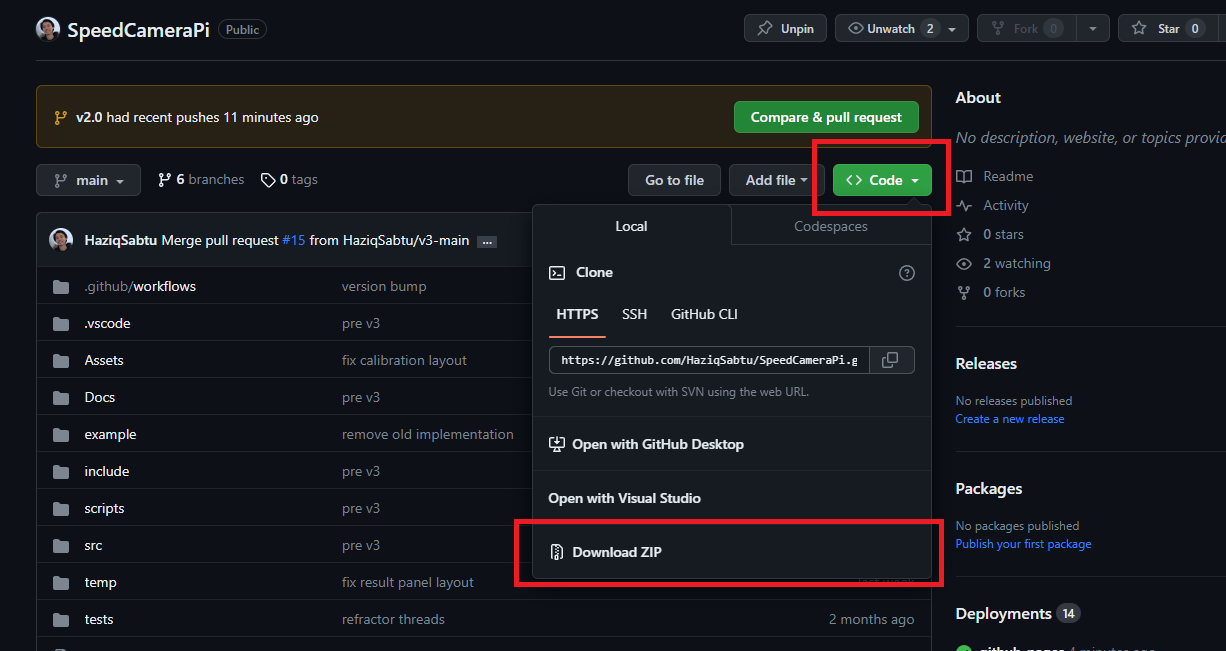
\includegraphics[width=0.65\textwidth]{texs/chapter1/image/dlcode.png}
            \end{figure}

      \item Extract the downloaded zip file to your \textbf{home} directory.
\end{itemize}

\section{Cloning the GitHub Repository}
\label{sec:cloning-the-github-repository}

Run the following commands to clone the repository:

\begin{lstlisting}
cd ~
git clone https://github.com/HaziqSabtu/SpeedCameraPi.git
\end{lstlisting}


\chapter{Installing Required Dependencies}
\label{chap:installing-required-dependencies}

In this chapter, we will be installing the required dependencies for the project. The dependencies are:

\begin{enumerate}
      \item OpenCV v4.5.5
      \item wxWidgets
      \item libcamera v0.0.4
\end{enumerate}

\section{Preparing the system}

Before installing the required dependencies, following steps are required to be done:

\begin{itemize}
      \item Navigate to scripts directory:

            \begin{lstlisting}
    cd ~/SpeedCameraPi/scripts/Installation
    \end{lstlisting}

      \item Allow script to be executed:

            \begin{lstlisting}
    sudo chmod +x DI_Scripts1.sh
    \end{lstlisting}

      \item Run script:

            \begin{lstlisting}
    sudo ./DI_Scripts1.sh
    \end{lstlisting}
\end{itemize}

\section{Preparing the system}

Before installing the required dependencies, following steps are required to be done:

\begin{itemize}
      \item Navigate to scripts directory:

            \begin{lstlisting}
    cd ~/SpeedCameraPi/scripts/Installation
    \end{lstlisting}

      \item Allow script to be executed:

            \begin{lstlisting}
    sudo chmod +x DI_Scripts1.sh
    \end{lstlisting}

      \item Run script:

            \begin{lstlisting}
    sudo ./DI_Scripts1.sh
    \end{lstlisting}
\end{itemize}

\subsection{Explanation of script}

\begin{itemize}
      \item Update the package list and upgrade all packages to their latest versions:

            \begin{lstlisting}
    sudo apt-get update && sudo apt-get upgrade
\end{lstlisting}

      \item Increase swap size to 4096MByte to prevent the system from running out of
            memory during the compilation process:

            \begin{lstlisting}
    NEW_SWAPSIZE=4096
    sudo sed -i "s/CONF_SWAPSIZE=.*/CONF_SWAPSIZE=$NEW_SWAPSIZE/" /etc/dphys-swapfile
    sudo sed -i "s/CONF_MAXSWAP=.*/CONF_MAXSWAP=$NEW_SWAPSIZE/" /sbin/dphys-swapfile
    sudo systemctl restart dphys-swapfile
\end{lstlisting}
\end{itemize}

\section{Installing OpenCV}

OpenCV is a powerful computer vision library that provides a vast range of image and video processing capabilities. This project uses OpenCV to perform image processing tasks such as detecting and tracking objects in the video stream.

Steps to install OpenCV on Raspberry Pi 4 running Debian: [\href{https://qengineering.eu/install-opencv-4.5-on-raspberry-pi-4.html}{source}]

\begin{itemize}
      \item Navigate to scripts directory:

            \begin{lstlisting}
    cd ~/SpeedCameraPi/scripts/Installation
    \end{lstlisting}

      \item Allow script to be executed:

            \begin{lstlisting}
    sudo chmod +x DI_Scripts2.sh
    \end{lstlisting}

      \item Run script:

            \begin{lstlisting}
    sudo ./DI_Scripts2.sh
    \end{lstlisting}
\end{itemize}

\section{Explanation of script}

\begin{itemize}
      \item Update the package list and upgrade all packages to their latest versions:

            \begin{lstlisting}
    sudo apt-get update && sudo apt-get upgrade
\end{lstlisting}

      \item Install the required dependencies for building OpenCV:

            \begin{lstlisting}
    sudo apt-get install -y build-essential cmake git unzip pkg-config
    sudo apt-get install -y libjpeg-dev libtiff-dev libpng-dev
    sudo apt-get install -y libavcodec-dev libavformat-dev libswscale-dev
    sudo apt-get install -y libgtk2.0-dev libcanberra-gtk* libgtk-3-dev
    sudo apt-get install -y libgstreamer1.0-dev gstreamer1.0-gtk3
    sudo apt-get install -y libgstreamer-plugins-base1.0-dev gstreamer1.0-gl
    sudo apt-get install -y libxvidcore-dev libx264-dev
    sudo apt-get install -y python3-dev python3-numpy python3-pip
    sudo apt-get install -y libtbb2 libtbb-dev libdc1394-22-dev
    sudo apt-get install -y libv4l-dev v4l-utils
    sudo apt-get install -y libopenblas-dev libatlas-base-dev libblas-dev
    sudo apt-get install -y liblapack-dev gfortran libhdf5-dev
    sudo apt-get install -y libprotobuf-dev libgoogle-glog-dev libgflags-dev
    sudo apt-get install -y protobuf-compiler
\end{lstlisting}

      \item Download OpenCV version 4.5.5 from the repository:

            \begin{lstlisting}
    cd ~ 
    sudo rm -rf opencv*
    wget -O opencv.zip https://github.com/opencv/opencarchive/4.5.5.zip 
    wget -O opencv_contrib.zip https://github.com/opencopencv_contrib/archive/4.5.5.zip 
    unzip opencv.zip 
    unzip opencv_contrib.zip 
    mv opencv-4.5.5 opencv
    mv opencv_contrib-4.5.5 opencv_contrib
    rm opencv.zip
    rm opencv_contrib.zip
\end{lstlisting}

      \item Create a build directory and navigate to it:

            \begin{lstlisting}
    cd ~/opencv
    mkdir build
    cd build
    \end{lstlisting}

      \item Configure the build process by running the following command:

            \begin{lstlisting}
    cmake -D CMAKE_BUILD_TYPE=RELEASE \
    -D CMAKE_INSTALL_PREFIX=/usr/local \
    -D OPENCV_EXTRA_MODULES_PATH=~/opencv_contrib/modules \
    -D ENABLE_NEON=ON \
    -D WITH_OPENMP=ON \
    -D WITH_OPENCL=OFF \
    -D BUILD_TIFF=ON \
    -D WITH_FFMPEG=ON \
    -D WITH_TBB=ON \
    -D BUILD_TBB=ON \
    -D WITH_GSTREAMER=ON \
    -D BUILD_TESTS=OFF \
    -D WITH_EIGEN=OFF \
    -D WITH_V4L=ON \
    -D WITH_LIBV4L=ON \
    -D WITH_VTK=OFF \
    -D WITH_QT=ON \
    -D OPENCV_ENABLE_NONFREE=ON \
    -D INSTALL_C_EXAMPLES=OFF \
    -D INSTALL_PYTHON_EXAMPLES=OFF \
    -D OPENCV_FORCE_LIBATOMIC_COMPILER_CHECK=1 \
    -D PYTHON3_PACKAGES_PATH=/usr/lib/python3/dist-packages \
    -D OPENCV_GENERATE_PKGCONFIG=ON \
    -D BUILD_EXAMPLES=OFF ..
    \end{lstlisting}

      \item Compile and install the library:

            \begin{lstlisting}
    make -j1
    sudo make install
    sudo ldconfig
\end{lstlisting}
\end{itemize}

\section{Installing wxWidget}

wxWidgets is a cross-platform GUI library that provides a set of C++ classes for
creating graphical user interfaces. This project uses wxWidgets to create the
graphical user interface for the application.

Steps to install wxWidget on Raspberry Pi 4 running Debian:
[\href{https://forums.raspberrypi.com/viewtopic.php?t=271709}{source}]

\begin{itemize}
      \item Navigate to scripts directory:

            \begin{lstlisting}
    cd ~/SpeedCameraPi/scripts/Installation
    \end{lstlisting}

      \item Allow script to be executed:

            \begin{lstlisting}
    sudo chmod +x DI_Scripts3.sh
    \end{lstlisting}

      \item Run script:

            \begin{lstlisting}
    sudo ./DI_Scripts3.sh
    \end{lstlisting}
\end{itemize}

\subsection{Explanation of script}

\begin{itemize}
      \item Update the package list and upgrade all packages to their latest versions:

            \begin{lstlisting}
    sudo apt-get update && sudo apt-get upgrade
    \end{lstlisting}

      \item Install the required dependencies for building wxWidgets:

            \begin{lstlisting}
    sudo apt-get install libgtk-3-dev build-essential checkinstall
    \end{lstlisting}

      \item Download the latest stable version of wxWidgets from the official website:

            \begin{lstlisting}
    wget https://github.com/wxWidgets/wxWidgets/releases/download/v3.2.2.1/wxWidgets-3.2.2.1.tar.bz2
    \end{lstlisting}

      \item Extract the downloaded archive and navigate to the extracted directory:

            \begin{lstlisting}
    tar -xvf wxWidgets-3.2.2.1.tar.bz2
    \end{lstlisting}

      \item Change directory to the extracted directory:

            \begin{lstlisting}
    cd wxWidgets-3.2.2.1
    \end{lstlisting}

      \item Create a build directory and navigate to it:

            \begin{lstlisting}
    mkdir gtk-build
    cd gtk-build
    \end{lstlisting}

      \item Configure the build process by running the following command:

            \begin{lstlisting}
    ../configure --disable-shared --enable-unicode --disable-debug
    \end{lstlisting}

      \item Compile and install the library:

            \begin{lstlisting}
    make
    sudo make install
    \end{lstlisting}

\end{itemize}

\subsection{Installing libcamera}

Libcamera is an open-source software stack designed to support complex camera configurations on Raspberry Pi and other embedded devices. It provides a unified interface for multiple camera modules, allowing developers to efficiently harness their full potential in various applications, from computer vision projects to advanced photography.

As of now, libcamera is still under development and is still in alpha stage. However, it is already being used by the Raspberry Pi Foundation to support the Raspberry Pi High-Quality Camera Module. It is recommended to use libcamera in the future as it provides a more flexible and powerful interface for controlling the camera module.

For this project, we will be using v0.0.4. As of now, a higher version is available, however, as it is still in the alpha stage, a lot of changes are still being made. When a more stable release is available, we will update this guide.

Steps to install Libcamera v0.0.4 on Raspberry Pi 4 running Debian:

\begin{itemize}
      \item Navigate to scripts directory:

            \begin{lstlisting}
    cd ~/SpeedCameraPi/scripts/Installation
    \end{lstlisting}

      \item Allow script to be executed:

            \begin{lstlisting}
    sudo chmod +x DI_Scripts4.sh
    \end{lstlisting}

      \item Run script:

            \begin{lstlisting}
    sudo ./DI_Scripts4.sh
    \end{lstlisting}
\end{itemize}

\subsection{Explanation of script}

\begin{itemize}
      \item Update the package list and upgrade all packages to their latest versions:

            \begin{lstlisting}
    sudo apt-get update && sudo apt-get upgrade
    \end{lstlisting}

      \item Install the required dependencies for building libcamera:

            \begin{lstlisting}
    sudo apt install -y libboost-dev
    sudo apt install -y libgnutls28-dev openssl libtiff5-dev pybind11-dev
    sudo apt install -y qtbase5-dev libqt5core5a libqt5gui5 libqt5widgets5
    sudo apt install -y meson
    sudo apt install -y cmake
    sudo pip3 install pyyaml ply
    sudo pip3 install --upgrade meson
    sudo apt install -y libglib2.0-dev libgstreamer-plugins-base1.0-dev
    \end{lstlisting}

      \item Download the repository and checkout to v0.0.4:

            \begin{lstlisting}
    cd ~
    git clone https://github.com/raspberrypi/libcamera.git
    cd libcamera
    git checkout v0.0.4
    \end{lstlisting}

      \item Configure and build the library:

            \begin{lstlisting}
    meson build --buildtype=release -Dpipelines=raspberrypi -Dipas=raspberrypi -Dv4l2=true -Dgstreamer=enabled -Dtest=false -Dlc-compliance=disabled -Dcam=disabled -Dqcam=enabled -Ddocumentation=disabled -Dpycamera=enabled
    ninja -C build -j2   # use -j 2 on Raspberry Pi 3 or earlier devices
    sudo ninja -C build install
    \end{lstlisting}

\end{itemize}

\subsection{Clean up}

After installing the required dependencies, you may want to clean up the unnecessary files to free up some disk space. To do so, run the following commands:

\begin{itemize}
      \item Navigate to scripts directory:

            \begin{lstlisting}
    cd ~/SpeedCameraPi/scripts/Installation
    \end{lstlisting}

      \item Allow script to be executed:

            \begin{lstlisting}
    sudo chmod +x DI_Scripts5.sh
    \end{lstlisting}

      \item Run script:

            \begin{lstlisting}
    sudo ./DI_Scripts5.sh
    \end{lstlisting}
\end{itemize}

\chapter{Compiling the Application}
\label{chap:compiling-the-application}

To build the application, follow these steps:

\begin{itemize}
      \item Create a build directory and navigate to it:

            \begin{lstlisting}
    cd ~/SpeedCameraPi
    mkdir build
    cd build
    \end{lstlisting}

      \item Configure the build process by running the following command:

            \begin{lstlisting}
    cmake -B. -H..
    \end{lstlisting}

      \item Compile the application:

            \begin{lstlisting}
    make -j3
    \end{lstlisting}

      \item After finished compiling, the executable file is located in the build directory.

            \begin{lstlisting}
    ./build
    \end{lstlisting}

      \item To run the application, simply double-click the executable file or run the following command:

            \begin{lstlisting}
    ./SpeedCameraPi
    \end{lstlisting}
\end{itemize}

\chapter{Utility Scripts}

This section will provide some useful scripts. These scripts are optional and are not required to run the application. However, they are useful for managing the application. The scripts are:

\begin{itemize}
      \item \textbf{Hotspot.sh} - This script will create a hotspot on the Raspberry Pi. This is useful if you want to connect to the Raspberry Pi without a router.
      \item \textbf{Startup.py} - This script will run the application on startup. This is useful if you want the application to run automatically when the Raspberry Pi boots up.
      \item \textbf{Touchscreen.sh} - This script will fix the Touchscreen rotation on the Raspberry Pi.
\end{itemize}

\section{Hotspot}

This script will configure the Raspberry Pi to enable the hotspot feature whenever it is not connected to the local network. This will allow you to connect to the Raspberry Pi directly when you are not at home.

\begin{itemize}
      \item Navigate to scripts directory:

            \begin{lstlisting}
    cd ~/SpeedCameraPi/scripts/Installation
    \end{lstlisting}

      \item Allow script to be executed:

            \begin{lstlisting}
    sudo chmod +x Hotspot.sh
    \end{lstlisting}

      \item Run script:

            \begin{lstlisting}
    sudo ./Hotspot.sh
    \end{lstlisting}
\end{itemize}

\section{Startup}

This script will configure the Raspberry Pi to automatically start the SpeedCameraPi application whenever it is booted up. This will allow you to use the Raspberry Pi as a standalone device without the need to manually start the application.

\begin{itemize}
      \item Navigate to scripts directory:

            \begin{lstlisting}
    cd ~/SpeedCameraPi/scripts/Installation
    \end{lstlisting}

      \item Allow script to be executed:

            \begin{lstlisting}
    sudo chmod +x Startup.py
    \end{lstlisting}

      \item Run script:

            \begin{lstlisting}
    sudo ./Startup.py
    \end{lstlisting}
\end{itemize}

\section{Touchscreen}

This script will fix the touchscreen rotation issue. This will allow you to use the touchscreen in portrait mode.

\begin{itemize}
      \item Navigate to scripts directory:

            \begin{lstlisting}
    cd ~/SpeedCameraPi/scripts/Installation
    \end{lstlisting}

      \item Allow script to be executed:

            \begin{lstlisting}
    sudo chmod +x Touchscreen.sh
    \end{lstlisting}

      \item Run script:

            \begin{lstlisting}
    sudo ./Touchscreen.sh
    \end{lstlisting}
\end{itemize}

\part{Setting up the Development Environment}

For future developers, this section will help you properly set up your
development environment. In general, the development is done with Visual Studio
Code with cross-compilation to Raspberry Pi 4. A guide to setting up the
development environment is provided below. Alternatively, a native development
setup will also be provided.

\chapter{Introduction}

C++ is a programming language that is designed to be compiled, meaning that it is
generally translated into machine language that can be understood directly by
the system, making the generated program highly efficient. To compile C++ code,
you need a set of tools known as the development toolchain, whose core are a
compiler and its linker. A compiler is a program that converts your C++ code
into machine code, while a linker is a program that combines the machine code
with other libraries and resources to create an executable file. There are
different compilers and linkers available for C++, such as Visual Studio, Clang,
mingw, etc. Some of them are integrated with IDEs (Integrated Development
Environments) that provide features such as syntax highlighting, debugging, code
completion, etc.

To cross-compile C++ code, you need to use a cross-compiler that can generate
executable code for a different platform than the one you are running on. For
example, if you want to compile C++ code for ARM architecture on a Windows PC,
you need to use a cross-compiler like arm-none-linux-gnueabi-gcc. Depending on the
tool you are using, you may need to configure some settings to enable cross
compilation. For example, if you are using Visual Studio Code, you can edit the
Compiler path and Compiler arguments settings in the C/C++ extension to specify
the cross-compiler and the target triplet. You can also use other tools like
CMake or Makefile to automate the cross-compilation process.

\chapter{Cross-compilation}

Cross-compilation is the process of compiling code on one platform (host) to run
on another platform (target). In this case, we will be compiling the code on a
Windows 11 machine running Windows Subsystem for Linux (WSL) to run on Raspberry
Pi 4 running Raspberry Pi OS (Bullseye 32-bit).

This method of development is preferred as it allows for faster compilation time
and easier debugging, which allows for better development experience.

Upon further reading, there are two important terms to take note of:

\begin{itemize}
      \item \textbf{Host} - The machine that you are developing on. In this case, it is the Windows 11 machine.
      \item \textbf{Target} - The machine that you are developing for. In this case, it is the Raspberry Pi 4.
\end{itemize}

This method has been tested numerous times and is proven to work. However, it is
not guaranteed to work on all machines. To reproduce the development
environment, following Build number of Windows 11 and WSL is required:

\begin{itemize}
      \item Windows 11 Pro Version 22H2 OS Build 22621.2428
      \item WSL 2 with Ubuntu 22.04 LTS
\end{itemize}

\section{Steps to setup Cross-Compilation}

For this section, it is assumed that you have already installed WSL 2 with
Ubuntu 22.04 LTS. If not, please refer to the
\href{https://docs.microsoft.com/en-us/windows/wsl/install-win10}{official documentation} to install WSL 2 with Ubuntu 22.04 LTS. Most of the process are taken from \href{https://github.com/abhiTronix/raspberry-pi-cross-compilers/wiki/Cross-Compiler-CMake-Usage-Guide-with-rsynced-Raspberry-Pi-32-bit-OS#cross-compiler-cmake-usage-guide-with-rsynced-raspberry-pi-32-bit-OS}{this guide}.

\begin{itemize}
      \item To begin with, it is important that required dependencies are installed on \textbf{Target}. Refer to the Section \ref{chap:installing-required-dependencies} to install the required dependencies.

      \item Next, we need to prepare the \textbf{Target} to allow ssh connection from the host. To do so, run the following command on \textbf{Host}:

            \begin{lstlisting}
        cd ~/SpeedCameraPi/scripts/crosscompile
        sudo chmod +x setup_ssh.py
        ./setup_ssh.py hostname username
    \end{lstlisting}

            Type yes when prompted. When successful, you should now be able to ssh into
            the target from the host with the following command:

            \begin{lstlisting}
        ssh RPi0
    \end{lstlisting}

      \item Next, we need to prepare the \textbf{target} for cross-compilation. To do so, run the following command on \textbf{Host}:

            \begin{lstlisting}
        cd ~/SpeedCameraPi/scripts/crosscompile
        sudo chmod +x Target_setup.py
        ./Target_setup.py credential password
    \end{lstlisting}

      \item Next, we need to prepare the \textbf{host} for cross-compilation. To do so, run the following command on \textbf{Host}:

            \begin{lstlisting}
        cd ~/SpeedCameraPi/scripts/crosscompile
        sudo chmod +x Host_setup.py
        sudo ./Host_setup.py
    \end{lstlisting}

      \item Lastly, now we need to sync the files structure of \textbf{Target} with \textbf{Host} on the staging directory (sysroot). To do so run following command:

            \begin{lstlisting}
        cd ~/SpeedCameraPi/scripts/crosscompile
        sudo chmod +x Host_postSetup.py
        ./Host_postSetup.py
    \end{lstlisting}

      \item Now, you should be able to perform cross-compilation. However, as of now, there is a linker problem with OpenCV libraries. To fix this, please refer to the next section.
\end{itemize}

\section{Fixing OpenCV linker problem}

Now, we will once again compile OpenCV. There seems to be a problem using the already compiled library of OpenCV as done previously on the \textbf{Target}. Some \textit{opencv\_contrib} libraries cannot be found during runtime. Possible linker error? Still investigating. However, the current fix is to cross compile the library on the \textbf{Host} and transfer the compiled libs to the \textbf{Target}.

\begin{itemize}
      \item To do
            so, follow these steps:

            \begin{lstlisting}
        cd ~/SpeedCameraPi/scripts/crosscompile
        sudo chmod +x Target_cvinstall.py
        ./Target_cvinstall.py credential
    \end{lstlisting}

      \item Now, we will compile OpenCV on \textbf{host} machine:

            \begin{lstlisting}
        cd ~/SpeedCameraPi/scripts/crosscompile
        sudo chmod +x Host_cvcompile.py
        sudo ./Host_cvcompile.py
    \end{lstlisting}

            In some cases, during compilation of OpenCV, it will produce error \textit{jconfig.h not found}. To fix this, run the following command:

            \begin{lstlisting}
        cd ~/SpeedCameraPi/scripts/crosscompile
        sudo chmod +x fix_jconfig.py
        ./fix_jconfig.py
    \end{lstlisting}

      \item Now, when the library is compiled, we can transfer the compiled library to the
            \textbf{target} machine. To do so, run the following command on \textbf{Host}:

            \begin{lstlisting}
        cd ~/SpeedCameraPi/scripts/crosscompile
        sudo chmod +x Host_cvinstall.py
        ./Host_cvinstall.py
    \end{lstlisting}

\end{itemize}

Now, the machine is ready for cross-compilation. Now we will explore steps to install Visual Studio Code.

\section{Installing Visual Studio Code}

Visual Studio Code is a free source-code editor made by Microsoft for Windows, Linux, and macOS. It is a very popular code editor among developers. This section will guide you through the process of installing Visual Studio Code for cross-compilation.

If you are running Linux on WSL, it is recommended to install Visual Studio Code directly on Windows. Download the installer from \href{https://code.visualstudio.com/Download}{here} and install it on Windows.

\section{Accessing WSL from Visual Studio Code}

First, we need to install the WSL Extension for Visual Studio Code. To do so, open the Extensions pane (Ctrl+Shift+X) and search for WSL. Click on the Install button to install the extension.

\begin{figure}[H]
      \centering
      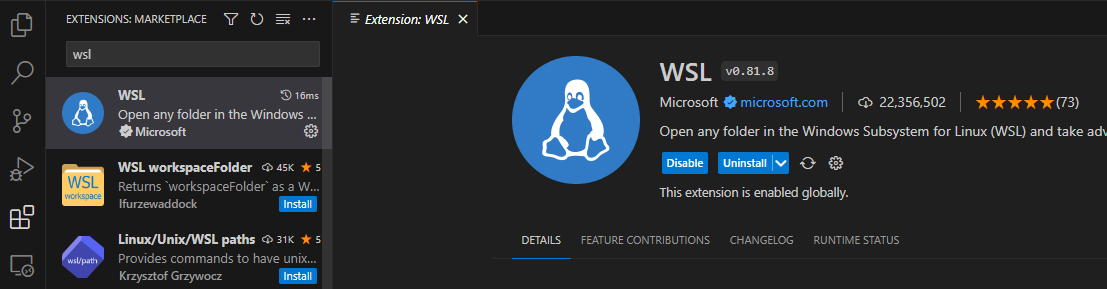
\includegraphics[width=0.8\textwidth]{texs/chapter1/image/wslext.png}
\end{figure}

To access WSL from Visual Studio Code, open the Command Palette (Ctrl+Shift+P) and type \texttt{WSL: Connect to WSL}. This will open a new Visual Studio Code window with WSL as the default shell. You can also open a folder in WSL by right-clicking on the folder in the File Explorer and selecting Open in WSL.

\begin{figure}[H]
      \centering
      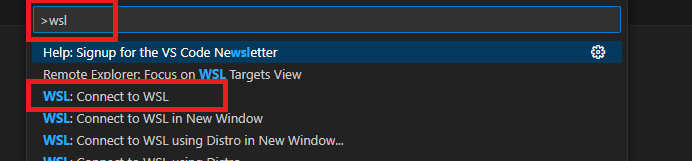
\includegraphics[width=0.8\textwidth]{texs/chapter1/image/wslconnect.png}
\end{figure}

You should see that you are currently in the WSL shell. You can also check the bottom left corner of the window to see if you are in the WSL shell.

\begin{figure}[H]
      \centering
      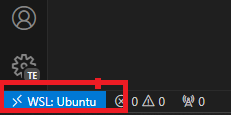
\includegraphics[width=0.8\textwidth]{texs/chapter1/image/wslconnect2.png}
\end{figure}

\section{Installing Required Extensions}

To install extensions, open Visual Studio Code and press Ctrl+Shift+X to open the Extensions pane. Search for the following extensions and install them:

\begin{itemize}
      \item C/C++ Extension Pack
\end{itemize}

\begin{figure}[H]
      \centering
      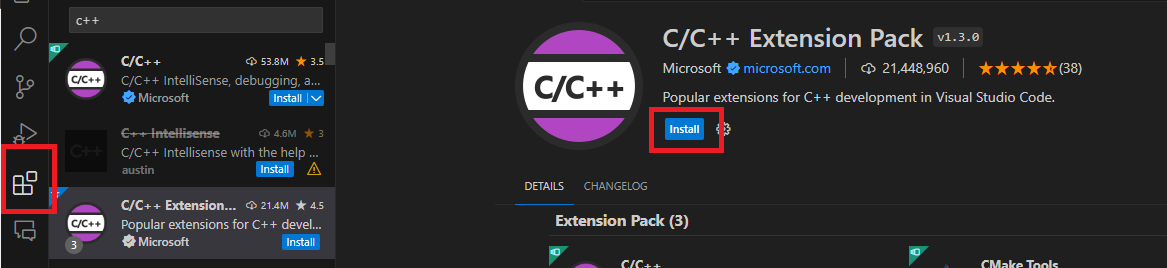
\includegraphics[width=0.8\textwidth]{texs/chapter1/image/c++ext.png}
\end{figure}

\section{Opening SpeedCameraPi project}

To open the SpeedCameraPi project, open the Explorer pane (Ctrl+Shift+E) and click on the Open Folder button. Navigate to the SpeedCameraPi folder and click on the OK button. You should now see the SpeedCameraPi project in the Explorer pane.

\begin{figure}[H]
      \centering
      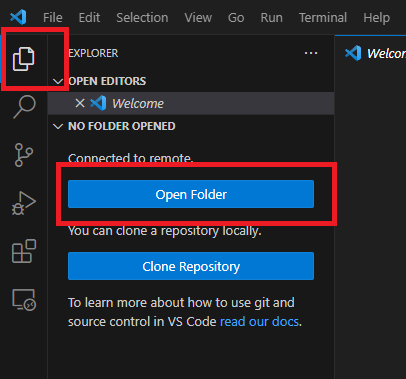
\includegraphics[width=0.8\textwidth]{texs/chapter1/image/wslfolder.png}
\end{figure}

\begin{figure}[H]
      \centering
      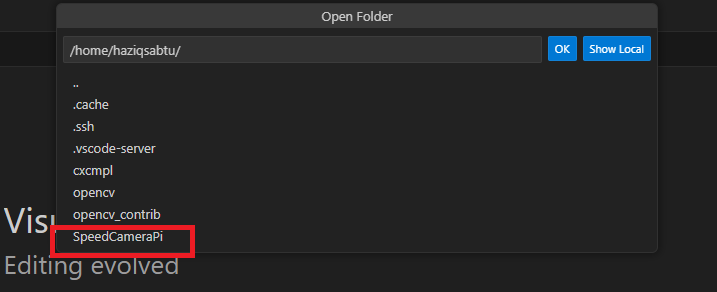
\includegraphics[width=0.8\textwidth]{texs/chapter1/image/wslfolder2.png}
\end{figure}

\section{Configuring C/C++ Extension}

To configure the C/C++ extension, open the Command Palette (Ctrl+Shift+P) and type \texttt{CMake:Configure} and select the \texttt{Pi Toolchain} option. This will create a \texttt{build} folder in the project directory and generate the CMake cache.

If the \texttt{Pi Toolchain} option is not available, you may need to check if the cross-compilation setup is done correctly. Additionally, in some cases the path may be different. If so, you may need to edit the \texttt{.vscode/cmake-kits.json} file to change the path to the cross compiler.

\begin{figure}[H]
      \centering
      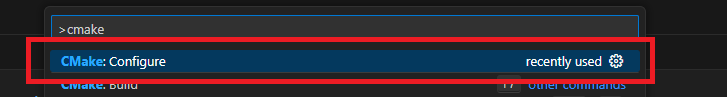
\includegraphics[width=0.8\textwidth]{texs/chapter1/image/cppconf.png}
\end{figure}

\begin{figure}[H]
      \centering
      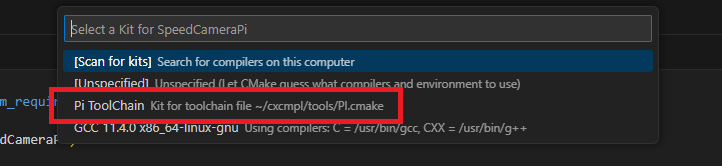
\includegraphics[width=0.8\textwidth]{texs/chapter1/image/cppconf2.png}
\end{figure}

If the configuration process is successful, you should see the following message in the terminal:

\begin{figure}[H]
      \centering
      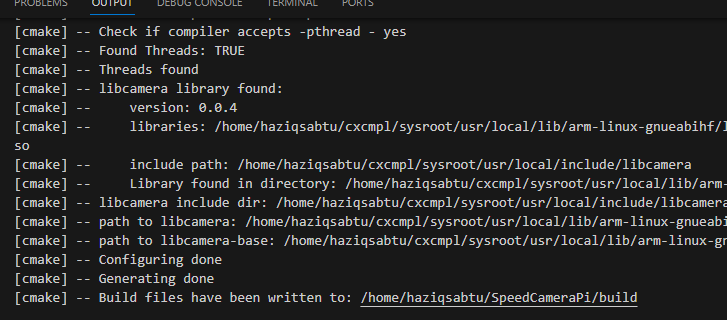
\includegraphics[width=0.8\textwidth]{texs/chapter1/image/cppconf3.png}
\end{figure}

\section{Building the project}

To build the project, open the Command Palette (Ctrl+Shift+P) and type \texttt{CMake:Build}. This will build the project and generate the executable file in the \texttt{build} folder.

\begin{figure}[H]
      \centering
      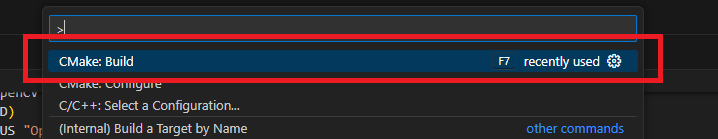
\includegraphics[width=0.8\textwidth]{texs/chapter1/image/cppbuild.png}
\end{figure}

Within the \texttt{CMakeLists.txt} file, the executable file is by default configured to be automatically copied to the \textbf{Target} machine. You can disable this by editing out the command. However, it is recommended to keep it as it is. The build application is located at \texttt{\~/Target/SpeedCameraPi}.

\section{Debugging the project}

\subsection{Preparations}

Debugging is crucial when developing a project. These steps need to be done at least once. To perform debugging, we first need to configure the \texttt{launch.json} script. To do so, navigate to the script folder:

\begin{lstlisting}
cd ~/SpeedCameraPi/scripts/debug
\end{lstlisting}

Next, run the following command:

\begin{lstlisting}
sudo chmod +x launch.py
\end{lstlisting}

Lastly, run the script with the following parameters:

\begin{lstlisting}
sudo ./launch.py ipaddress
\end{lstlisting}

This will generate the \texttt{launch.json} file in the \texttt{.vscode} folder. Now we need to install \texttt{gdbserver} on the \textbf{Target} machine. To do so, run the following command on \textbf{Host}:

\begin{lstlisting}
ssh RPi0
sudo apt-get install gdbserver
\end{lstlisting}

\subsection{Debugging}

To debug the project, open the Debugger Tab (\texttt{Ctrl + Shift + D}) and select the profile \texttt{(GDB-Auto) Remote GDB Launch} and click on the Run button. This will start the \texttt{gdbserver} on the \textbf{Target} machine and connect to it. You should now be able to debug the project.

\begin{figure}[H]
      \centering
      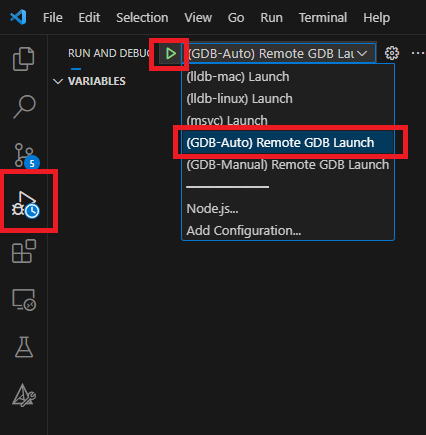
\includegraphics[width=0.8\textwidth]{texs/chapter1/image/debug.png}
\end{figure}

\subsection{Known Issues}

In some cases, certain libraries cannot be found. To fix this, run the following command on \textbf{Host}:

\begin{itemize}
      \item \texttt{libncurses.so}
            \begin{lstlisting}
    sudo apt install libncurses5
    \end{lstlisting}

      \item \texttt{libpython2.7.so}
            \begin{lstlisting}
    sudo apt install libpython2.7
    \end{lstlisting}
\end{itemize}

\section{Extra Features}

In this section, we will explore some extra features that can be used to improve the development experience.

\subsection{VNC Viewer}

VNC Viewer is a remote desktop application that allows you to remotely control a computer. It is useful for accessing the \textbf{Target} machine remotely. By properly integrating the VNC, your Raspberry Pi can be used without a monitor, keyboard, or mouse.

To download VNC Viewer, go to \href{https://www.realvnc.com/en/connect/download/viewer/}{this link} and download the installer for your operating system. Once installed, you may need to create an account to use the application. Once done you may need to prepare the \textbf{Target} machine to allow VNC connection. To do so, run the following command on \textbf{Host}:

\begin{lstlisting}
ssh RPi0
sudo raspi-config
\end{lstlisting}

Navigate to \textbf{Interface Options} and enable \textbf{VNC}.

\begin{figure}[H]
      \centering
      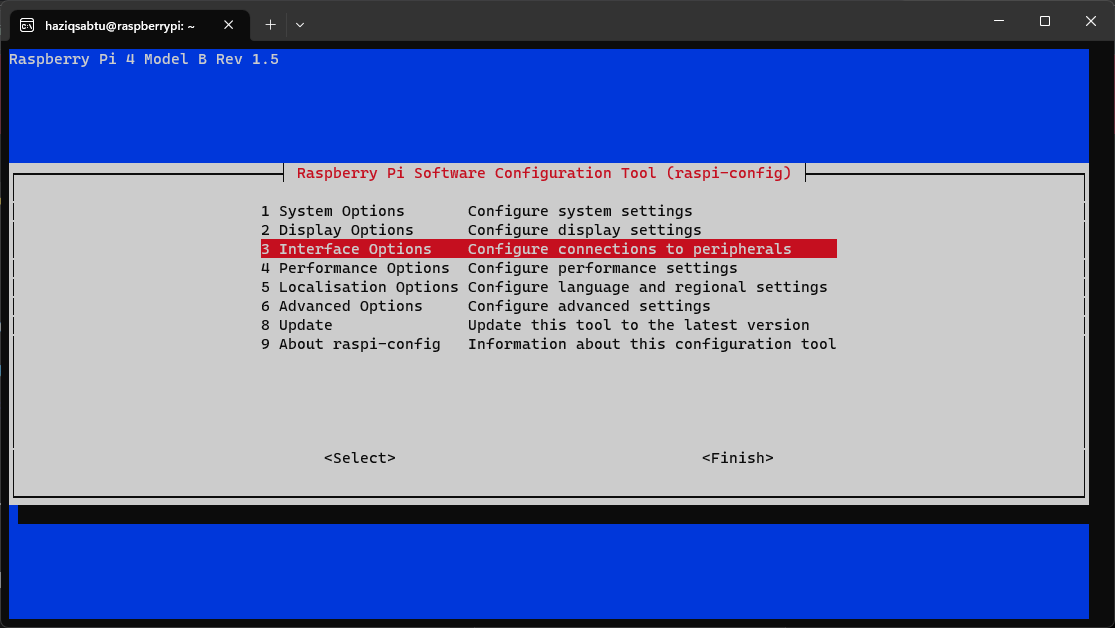
\includegraphics[width=0.8\textwidth]{texs/chapter1/image/vnc1.png}
\end{figure}

\begin{figure}[H]
      \centering
      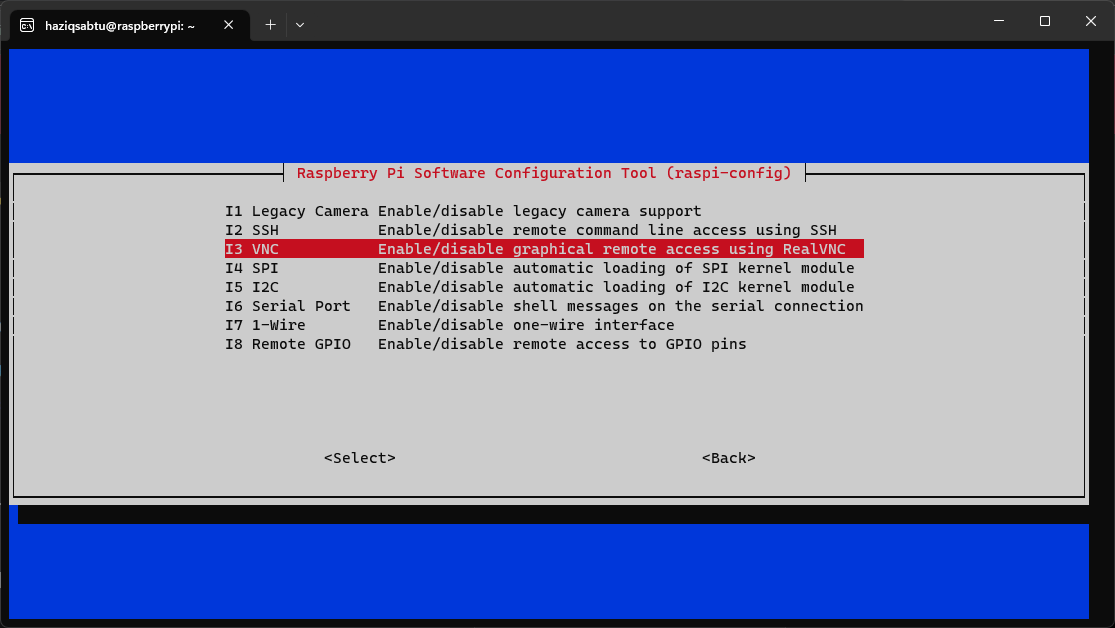
\includegraphics[width=0.8\textwidth]{texs/chapter1/image/vnc2.png}
\end{figure}

\begin{figure}[H]
      \centering
      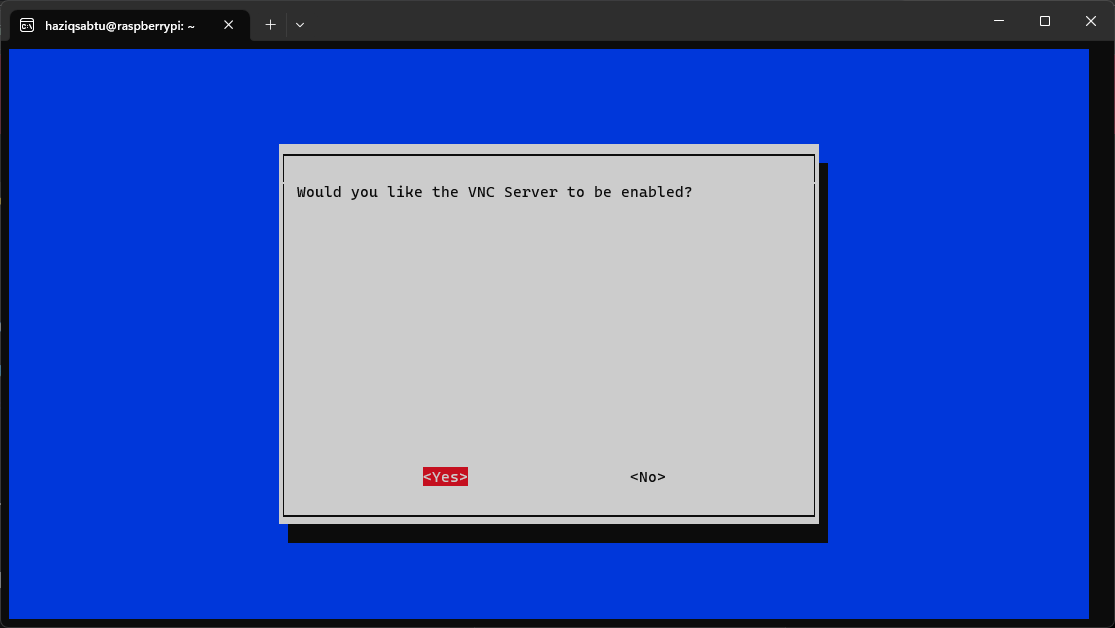
\includegraphics[width=0.8\textwidth]{texs/chapter1/image/vnc3.png}
\end{figure}

Now, you should be able to access the \textbf{Target} machine via VNC Viewer. It is recommended to reboot the \textbf{Target} machine after enabling VNC.

To access the \textbf{Target} machine via VNC Viewer, you need to know the IP address of the \textbf{Target} machine. To do so, run the following command on \textbf{Host}:

\begin{lstlisting}
hostname -I
\end{lstlisting}

Alternatively, it is defaulted to \texttt{raspberrypi}.

Now, you can access the \textbf{Target} machine via VNC Viewer. To do so, open VNC Viewer and create a new connection (\texttt{Ctrl + N}) and set the following parameters:

\begin{itemize}
      \item \textbf{VNC Server} - IP address of the \textbf{Target} machine
      \item \textbf{Name} - Name of the connection, can be anything
\end{itemize}

\begin{figure}[H]
      \centering
      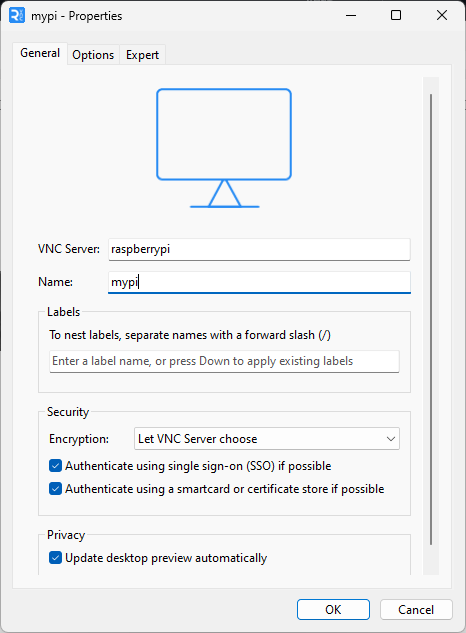
\includegraphics[width=0.8\textwidth]{texs/chapter1/image/vnc4.png}
\end{figure}

Now, you should be able to access the \textbf{Target} machine via VNC Viewer. You may need to enter the password of the \textbf{Target} machine.

\subsection{VSCode Extensions}

Following are some useful extensions that can be used to improve the development experience:

\begin{itemize}
      \item \href{https://marketplace.visualstudio.com/items?itemName=xaver.clang-format}{Clang-Format}: Clang-Format is a tool that formats C/C++/Obj-C code according to a set of style options, similar to the way that clang-format formats code.
      \item \href{https://marketplace.visualstudio.com/items?itemName=GitHub.copilot}{Github Copilot}: GitHub Copilot is an AI pair programmer that helps you write code faster and with less work.
      \item \href{https://marketplace.visualstudio.com/items?itemName=Gruntfuggly.todo-tree}{Todo Tree}: Todo Tree is a task manager that helps you manage your TODOs.
\end{itemize}

\chapter{Native Compilation}

For those who prefer to develop natively on the Raspberry Pi, this section will guide you through the process of setting up the development environment.

For native compilation, the steps are much simpler. Simply install the required dependencies on the \textbf{Target} machine and you are good to go. Refer to \href{md_Docs_markdown_InstallingRequiredDependency.html}{this section} for more information.

The installation of VSCode on Raspberry Pi is done with \href{https://code.visualstudio.com/docs/setup/raspberry-pi}{this} instruction.

\section{Installing required Extensions}

To install extensions, open Visual Studio Code and press \texttt{Ctrl+Shift+X} to open the Extensions pane. Search for the following extensions and install them:

\begin{itemize}
      \item C/C++ Extension Pack
\end{itemize}

\begin{figure}[H]
      \centering
      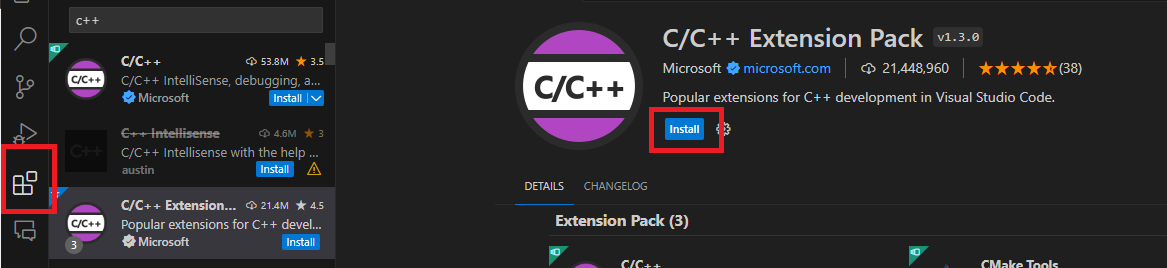
\includegraphics[width=0.8\textwidth]{texs/chapter1/image/c++ext.png}
\end{figure}

\section{Opening SpeedCameraPi project}

To open the SpeedCameraPi project, open the Explorer pane (\texttt{Ctrl+Shift+E}) and click on the Open Folder button. Navigate to the SpeedCameraPi folder and click on the OK button. You should now see the SpeedCameraPi project in the Explorer pane.

\begin{figure}[H]
      \centering
      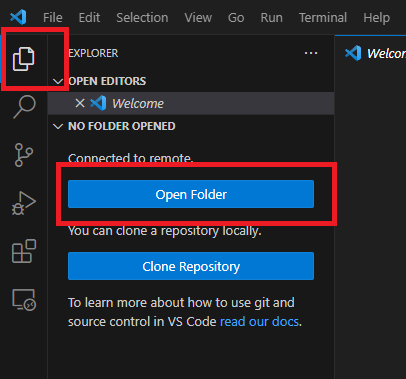
\includegraphics[width=0.8\textwidth]{texs/chapter1/image/wslfolder.png}
\end{figure}

\begin{figure}[H]
      \centering
      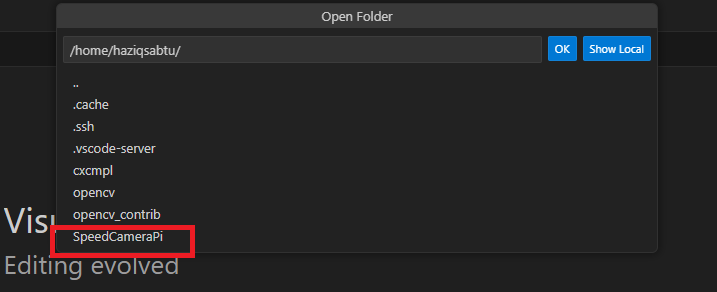
\includegraphics[width=0.8\textwidth]{texs/chapter1/image/wslfolder2.png}
\end{figure}

\section{Configuring C/C++ extension}

To configure the C/C++ extension, open the Command Palette (\texttt{Ctrl+Shift+P}) and type \texttt{CMake:Configure} and select the default compiler. This will create a \texttt{build} folder in the project directory and generate the CMake cache.

\begin{figure}[H]
      \centering
      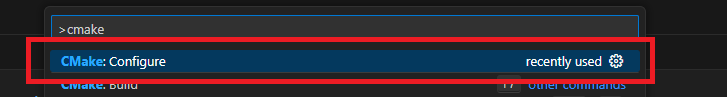
\includegraphics[width=0.8\textwidth]{texs/chapter1/image/cppconf.png}
\end{figure}

\begin{figure}[H]
      \centering
      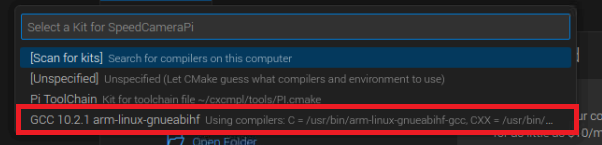
\includegraphics[width=0.8\textwidth]{texs/chapter1/image/cppconf4.png}
\end{figure}

If the configuration process is successful, you should see the following message in the terminal:

\begin{figure}[H]
      \centering
      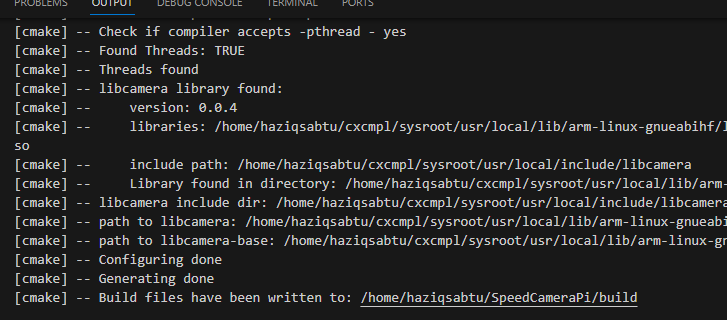
\includegraphics[width=0.8\textwidth]{texs/chapter1/image/cppconf3.png}
\end{figure}

\section{Building the project}

To build the project, open the Command Palette (\texttt{Ctrl+Shift+P}) and type \texttt{CMake:Build}. This will build the project and generate the executable file in the \texttt{build} folder.

\begin{figure}[H]
      \centering
      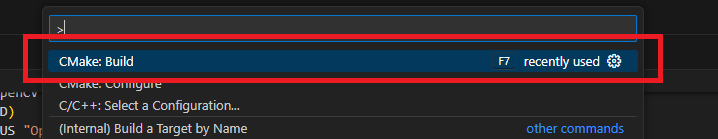
\includegraphics[width=0.8\textwidth]{texs/chapter1/image/cppbuild.png}
\end{figure}

If the UI is unresponsive, it is highly likely that the building process is using all of the resources available. Either wait until the process completes, or reduce the number of parallel build jobs. To do so, open the Command Palette (\texttt{Ctrl+Shift+P}) and type \texttt{Settings: Open Settings (UI)}. Navigate to \texttt{CMake: Parallel Jobs} and set the value to 1.

\begin{figure}[H]
      \centering
      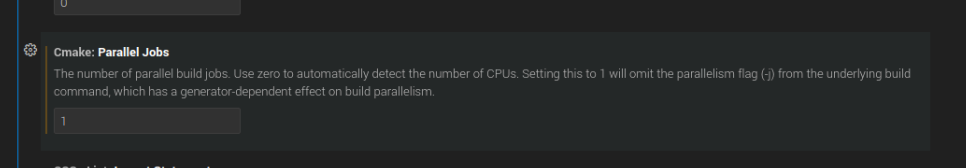
\includegraphics[width=0.8\textwidth]{texs/chapter1/image/cppbuild3.png}
\end{figure}

\section{Debugging}

To debug the project, open the Debugger Tab (\texttt{Ctrl + Shift + D}) and select the profile \texttt{GDB - Native} and click on the Run button. This will compile the project and start the debugger. You should now be able to debug the project.

\begin{figure}[H]
      \centering
      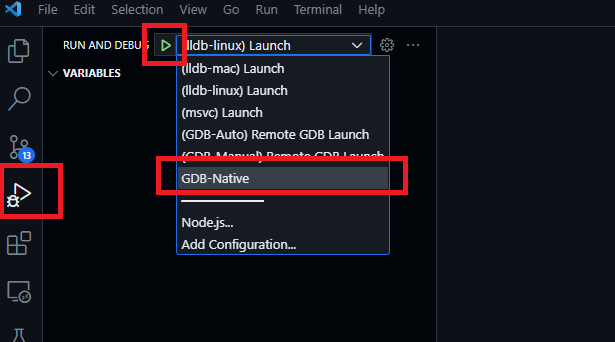
\includegraphics[width=0.8\textwidth]{texs/chapter1/image/debug2.png}
\end{figure}

\part{Getting Started with Development}

\chapter{Introduction}

This section will guide you through the process of developing the application. It is assumed that you have already set up the development environment. If not, please refer to the previous section. This section will cover the following topics:

\begin{itemize}
      \item \textbf{Adding a new Panel} - This section will guide you through the process of adding a new panel to the application.
      \item \textbf{Custom Event} - This section will guide you through the process of defining, triggering, and handling custom events.
      \item \textbf{Defining Process Threads} - This section will guide you through the process of defining process threads.
      \item \textbf{Creating Tasks} - This section will guide you through the process of creating tasks for ThreadPool.
\end{itemize}

\chapter{Add new Panel}

This chapter will provide description on how to add new panel to the application. To add a new Panel to the Application, following steps are required:
\begin{enumerate}
      \item Define a new PanelID Enum
      \item Create a new Controller class
      \item Create a new Panel class
      \item Define object in MainFrame
\end{enumerate}

\section{Define a new PanelID Enum}

The first step is to register a unique enum for the Panel. This enum will be used to identify the Panel in the application. To add a new Panel enum, modify the PanelID enum in the \texttt{include/Model/Enum.hpp} file. Following example will provide a simple example of a PanelID enum:

\begin{lstlisting}[language=C++, caption={PanelID enum example}]
enum PanelID {
    // ... other enum
    PANEL_INFO,
    PANEL_MY_PANEL, // Add new PanelID enum here
};
\end{lstlisting}

\section{Create a new Controller class}

\subsection{Define a new Controller class}

To create a new controller class, you first need to decide either the Panel will require a touch input or not. If touch input is required you can create a custom controller class that extends the BaseControllerWithTouch class. Otherwise you can create a custom controller class that extends the BaseController class. Following example will provide a simple example of a Controller class that extends the BaseControllerWithTouch class:

\begin{lstlisting}[language=C++, caption={MyController class example}]
class MyController : public BaseControllerWithTouch {
  public:
    MyController(ResourcePtr shared);
    ~MyController();

  private:
    static const PanelID currentPanelID = PanelID::PANEL_MY_PANEL; // Add new PanelID enum here

  private:
    void throwIfAnyThreadIsRunning() override;

    void killAllThreads(wxEvtHandler *parent) override;

    void leftDownHandler(wxEvtHandler *parent, cv::Point point) override;
    void leftMoveHandler(wxEvtHandler *parent, cv::Point point) override;
    void leftUpHandler(wxEvtHandler *parent, cv::Point point) override;
};
\end{lstlisting}

Make sure that you implemented the pure virtual functions from the BaseControllerWithTouch class. The pure virtual functions are:
\begin{itemize}
      \item \texttt{void throwIfAnyThreadIsRunning() override;}
      \item \texttt{void killAllThreads(wxEvtHandler *parent) override;}
      \item \texttt{void leftDownHandler(wxEvtHandler *parent, cv::Point point) override;}
      \item \texttt{void leftMoveHandler(wxEvtHandler *parent, cv::Point point) override;}
      \item \texttt{void leftUpHandler(wxEvtHandler *parent, cv::Point point) override;}
\end{itemize}

See the source code for \texttt{LaneCalibrationController} for example.

To make the code more readable, it is advised to define the controller shared pointer to a shorter name. Following example will provide a simple example of defining a shorter name for the Controller shared pointer:

\begin{lstlisting}[language=C++, caption={Shorter name for Controller shared pointer}]
#define MCPtr std::shared_ptr<MyController>
\end{lstlisting}

\subsection{Add method to ControllerFactory}

The \texttt{ControllerFactory} is used to connect the Controller with the Model component. Following example can be used:

\begin{lstlisting}[language=C++, caption={ControllerFactory method example}]
class ControllerFactory {
  public:
    ControllerFactory(wxWindow *parent);
    ~ControllerFactory();

    ResourcePtr getSharedModel();

    // ... other methods
    MyPtr createMyController();

  private:
    ResourcePtr shared;
};
\end{lstlisting}

\begin{lstlisting}[language=C++, caption={Implementation of createMyController method}]
MyPtr ControllerFactory::createMyController() {
    return std::make_shared<MyController>(shared);
}
\end{lstlisting}

\section{Create a new Panel class}

\subsection{Define a new Panel class}

To create a new Panel class, you need to create a new class that extends either the BasePanel or the BasePanelWithTouch class. The BasePanel class has already implemented the basic functionality of a Panel, while the BasePanelWithTouch class has already implemented the basic functionality of a Panel with touch support. The BasePanelWithTouch class is recommended to be used if the Panel will be used in a touch screen device. Alternatively you can also create a whole new class that extends the wxPanel class from wxWidgets. Following example will provide a simple example of a Panel class that extends the BasePanelWithTouch class:

\begin{lstlisting}[language=C++, caption={MyPanel class example}]
class MyPanel : public BasePanelWithTouch {
  public:
    MyPanel(wxWindow *parent, wxWindowID id, MyPtr controller);
    ~MyPanel();

  private:
    const PanelID panel_id = PANEL_MY_PANEL;

    MyPtr controller;

    DECLARE_EVENT_TABLE()
};
\end{lstlisting}

Make sure that if you are using the BasePanelWithTouch class, you are also using the BaseControllerWithTouch class. Otherwise you will get a compilation error.

\subsection{Create ButtonPanel}

Now create a ButtonPanel for the Panel. The ButtonPanel is a panel that contains buttons to perform certain actions. To create a ButtonPanel, you need to create a new class that extends the BaseButtonPanel class. Following example will provide a simple example of a ButtonPanel class that extends the BaseButtonPanel class:

\begin{lstlisting}[language=C++, caption={CustomButtonPanel class example}]
class CustomButtonPanel : public BaseButtonPanel {
  public:
    CustomButtonPanel(wxWindow *parent, wxWindowID id);

    void update(const AppState &state) override;

    // define all buttons here

    DECLARE_EVENT_TABLE();
};
\end{lstlisting}

Make sure that the \texttt{update()} method is implemented. The \texttt{update()} method will be called by the Panel to update the state of the buttons.

\subsection{Implement the Panel class}

Now that you have created the ButtonPanel, you can now implement the Panel class. Following example can be used as a reference to implement the Panel class:

\begin{lstlisting}[language=C++, caption={Implementation of MyPanel class}]
MyPanel::MyPanel(wxWindow *parent, wxWindowID id,
                                           MyPtr controller)
    : BasePanelWithTouch(parent, id, controller), controller(controller) {

    button_panel =
        new CustomButtonPanel(this, wxID_ANY);
    title_panel = new TitlePanel(this, panel_id);

    size();
}
\end{lstlisting}

Make sure the \texttt{size()} method is called at the end of the constructor. The \texttt{size()} method will set the sizer of the Panel.

\subsection{Add method to PanelFactory}

In this step, you need to modify the PanelFactory class. Following example can be used:

\begin{lstlisting}[language=C++, caption={Create Panel method in PanelFactory}]
wxPanel *createPanel(wxWindow *parent, PanelID panelID) {
        // ... other if case

        if (panelID == PANEL_MY_PANEL) {
            return createMyPanel(parent);
        }
    }

MyPanel *createMyPanel(wxWindow *parent) {
        return new MyPanel(parent, wxID_ANY, controllerFactory->createMyController());
    }
\end{lstlisting}

\section{Define object in MainFrame}

The last step is to define the Panel in the MainFrame class. Following example can be used:

\begin{lstlisting}[language=C++, caption={MainFrame class example}]
class MainFrame : public wxFrame {
    // ... other methods

    private:
    // ... other methods
    MyPanel *myPanel;
    // ... other methods
};

MainFrame::MainFrame() : wxFrame(NULL, wxID_ANY, Data::AppName) {

    // ... other methods

    // ... other registerPanel
    registerPanel(PANEL_MY_PANEL);

    showFirstPanel();
}
\end{lstlisting}

Now you have successfully added a new Panel to the application.

\chapter{Custom Event}

Events are used as a response mechanism for the View component. There are two types of events in this application:
\begin{itemize}
      \item DataEvent
      \item EmptyEvent
\end{itemize}

\section{DataEvent}

DataEvent is an event that contains data. The data can be any type of data. To create a new DataEvent, you need to create a new class that extends the \texttt{wxCommandEvent} class. Following example will provide a simple example of a DataEvent class:

\begin{lstlisting}[language=C++, caption={CustomEvent class example}]
class CustomEvent;
wxDECLARE_EVENT(c_CUSTOM_EVENT, CustomEvent);

enum CUSTOM_EVENT_TYPE {
    CUSTOM_EVENT_TYPE_1 = 1,
    CUSTOM_EVENT_TYPE_2,
    CUSTOM_EVENT_TYPE_3,
};

class CustomEvent : public wxCommandEvent {
  public:
    CustomEvent(wxEventType type, int id = 1);

    CustomEvent(const CustomEvent &event);
    virtual wxEvent *Clone() const override;

    // Define set and get method for the data here
    void setData(const std::string &data);
    std::string getData() const;

  private:
    std::string data;
};

// this part is important
typedef void (wxEvtHandler::*CustomFunction)(CustomEvent &);
#define CustomHandler(func)                                             \
    wxEVENT_HANDLER_CAST(CustomFunction, func)
#define EVT_CUSTOM(id, func)                                           \
    wx__DECLARE_EVT1(c_CUSTOM_EVENT, id, CustomHandler(func))
\end{lstlisting}

\begin{lstlisting}[language=C++, caption={CustomEvent continued}]
wxDEFINE_EVENT(c_CUSTOM_EVENT, CustomEvent);

CustomEvent::CustomEvent(wxEventType type, int id)
    : wxCommandEvent(type, id) {
}

CustomEvent::CustomEvent(const CustomEvent &event)
    : wxCommandEvent(event) {
    this->setData(event.getData());
}

wxEvent *UpdatePreviewEvent::Clone() const {
    return new CustomEvent(*this);
}

void CustomEvent::setData(const std::string &data) {
    this->data = data;
}

std::string CustomEvent::getData() const {
    return data;
}
\end{lstlisting}

\subsection{Example Classes}
The following classes can be referred to as examples:
\begin{itemize}
      \item UpdatePreviewEvent
      \item UpdateStateEvent
      \item ErrorEvent
\end{itemize}

\section{EmptyEvent}

EmptyEvent is an event that does not contain any data. It is normally used to signal the View component to perform certain action. To create a new EmptyEvent, you need to create a new class that extends the \texttt{wxCommandEvent} class. Following example will provide a simple example of an EmptyEvent class:

\begin{lstlisting}[language=C++, caption={EmptyEvent class example}]
wxDECLARE_EVENT(c_CUSTOM_EVENT, wxCommandEvent);

enum CUSTOM_EVENT_TYPE {
    CUSTOM_EVENT_TYPE_1 = 1,
    CUSTOM_EVENT_TYPE_2,
    CUSTOM_EVENT_TYPE_3,
};
\end{lstlisting}

\begin{lstlisting}[language=C++, caption={EmptyEvent continued}]
wxDEFINE_EVENT(c_CUSTOM_EVENT, wxCommandEvent);
\end{lstlisting}

\section{Bind Event}

To bind an event to a method, you need to use the following syntax in the Panel class:

\begin{lstlisting}[language=C++, caption={Binding Event in Panel class}]
BEGIN_EVENT_TABLE(BasePanel, wxPanel)
    // ... other event

    // For EmptyEvent
    EVT_COMMAND(wxID_ANY, c_CUSTOM_EVENT, BasePanel::OnCustomEvent)

    // For DataEvent
    EVT_CUSTOM(c_CUSTOM_EVENT, BasePanel::OnCustomEvent)
END_EVENT_TABLE()
\end{lstlisting}

Make sure the function to handle the event is implemented.

\section{Submit Event}

To submit an event, you need to use the following syntax:

\begin{lstlisting}[language=C++, caption={Submitting Event}]
// For EmptyEvent
wxCommandEvent event(c_CUSTOM_EVENT, CUSTOM_EVENT_TYPE_1);
wxPostEvent(this, event);

// For DataEvent
CustomEvent event(c_CUSTOM_EVENT, CUSTOM_EVENT_TYPE_1);
event.setData("data");
wxPostEvent(this, event);
\end{lstlisting}

\chapter{Thread}

Thread is used to perform a long-running task.

\section{Define unique ThreadID}

To define a unique ThreadID, you need to modify the ThreadID enum in the \texttt{include/Thread/Thread\_ID.hpp} file. Following example will provide a simple example of a ThreadID enum:

\begin{lstlisting}[language=C++, caption={ThreadID enum example}]
enum ThreadID {
    // ... other enum
    THREAD_MY_THREAD, // Add new ThreadID enum here
};
\end{lstlisting}

\section{Create a new Thread class}

Now you need to create a new class that extends the \texttt{BaseThread} class. Following example will provide a simple example of a Thread class:

\begin{lstlisting}[language=C++, caption={CustomThread class example}]
class CustomThread : public BaseThread {
  public:
    CustomThread(wxEvtHandler *parent, DataPtr data);
    ~CustomThread();

    ThreadID getID() const override;

  protected:
    virtual ExitCode Entry() override;

  private:
    // ... other methods
    const ThreadID thread_id = ThreadID::THREAD_MY_THREAD; // Add new ThreadID enum here
};

CustomThread::CustomThread(wxEvtHandler *parent, DataPtr data)
    : BaseThread(parent, data) {
}

CustomThread::~CustomThread() {
}

ThreadID CustomThread::getID() const {
    return thread_id;
}

wxThread::ExitCode CustomThread::Entry() {
    // ... other code, do process
    return (wxThread::ExitCode)0;
}
\end{lstlisting}

Additionally, following classes can be inherited to add more functionality:

\begin{table}[h]
      \centering
      \begin{tabular}{|l|p{10cm}|}
            \hline
            Class               & Description                                                              \\
            \hline
            PreviewableThread   & Enable the thread to send image to ImagePanel                            \\
            ImageSizeDataThread & Add variable \texttt{imageSize}, which is the size of the captured image \\
            ImageDataThread     & Add variable \texttt{image}, which is the camera                         \\
            CameraAccessor      & Enable camera access                                                     \\
            \hline
      \end{tabular}
\end{table}

\section{Add method to ThreadController}

In this step, you need to modify the \texttt{ThreadController} class. Following example can be used:

\begin{lstlisting}[language=C++, caption={ThreadController class example}]
class ThreadController {
  public:
    ThreadController(wxEvtHandler *parent, DataPtr data);
    ~ThreadController();

    // ... other methods

    virtual void startCustomThread(wxEvtHandler *parent, PanelID panelID);

    void endCustomThread();

    CustomThread *getCustomThread();

  private:
    // ... other variables 
    CustomThread *custom_thread;
};
\end{lstlisting}

\chapter{Task for ThreadPool}

ThreadPool enables parallel processing, which can be used to speed up the application. To add a new Task to the ThreadPool, following steps are required:

\section{Define unique TaskType}

To define a unique TaskType, you need to modify the TaskType enum in the \texttt{include/Thread/Task/Task.hpp} file. Following example will provide a simple example of a TaskType enum:

\begin{lstlisting}[language=C++, caption={TaskType enum example}]
enum TaskType {
    // ... other enum
    TASK_MY_TASK, // Add new TaskType enum here
};
\end{lstlisting}

\section{Create a new Task class}

Now you need to create a new class that extends the Task class. Following example will provide a simple example of a Task class:

\begin{lstlisting}[language=C++, caption={CustomTask class example}]
class CustomTask : public Task {
  public:
    CustomTask(wxEvtHandler *parent, DataPtr data);
    void Execute() override;

  private:
    // ... other methods
    const std::string currentName = "CustomTask";
    const TaskType currentType = TaskType::TASK_MY_TASK; // Add new TaskType enum here
};

CustomTask::CustomTask(wxEvtHandler *parent, DataPtr data)
    : Task(parent, data) {
    property = TaskProperty(currentType);
    name = currentName;
}

void CustomTask::Execute() {
    // ... other code, do process
}
\end{lstlisting}


